\documentclass{beamer}
\usepackage{amssymb,amsmath,amsfonts,pdfpages,color, url}
\usepackage{booktabs}
\usepackage{wrapfig}
\usepackage{amsmath}
\usepackage{multirow}

\setbeamertemplate{navigation symbols}{}
\usetheme{Montpellier}

\setbeamertemplate{footline}[page number]


\def\dis{\mathop{\displaystyle}}
\def\argmin{\mathop{\rm argmin}}


\newcommand{\E}{\mathbb{E}}
\newcommand{\jeff}[1]{{\color{blue}$\langle$Jeff: #1$\rangle$}}
\newcommand{\dgen}{\ensuremath{\mathtt{d}}}



\title{Scalable Personalised Item Ranking through Parametric Density Estimation}
\author{Riku Togashi, Masahiro Kato, Mayu Otani, Tetsuya Sakai and Shin'ichi Satoh}
\institute{SIGIR '21, July 11--15, 2021}
\date{}

\begin{document}

\frame{\titlepage}


\section{Motivation}

\begin{frame}
\frametitle{Problem Definition}
\begin{figure}[h] 
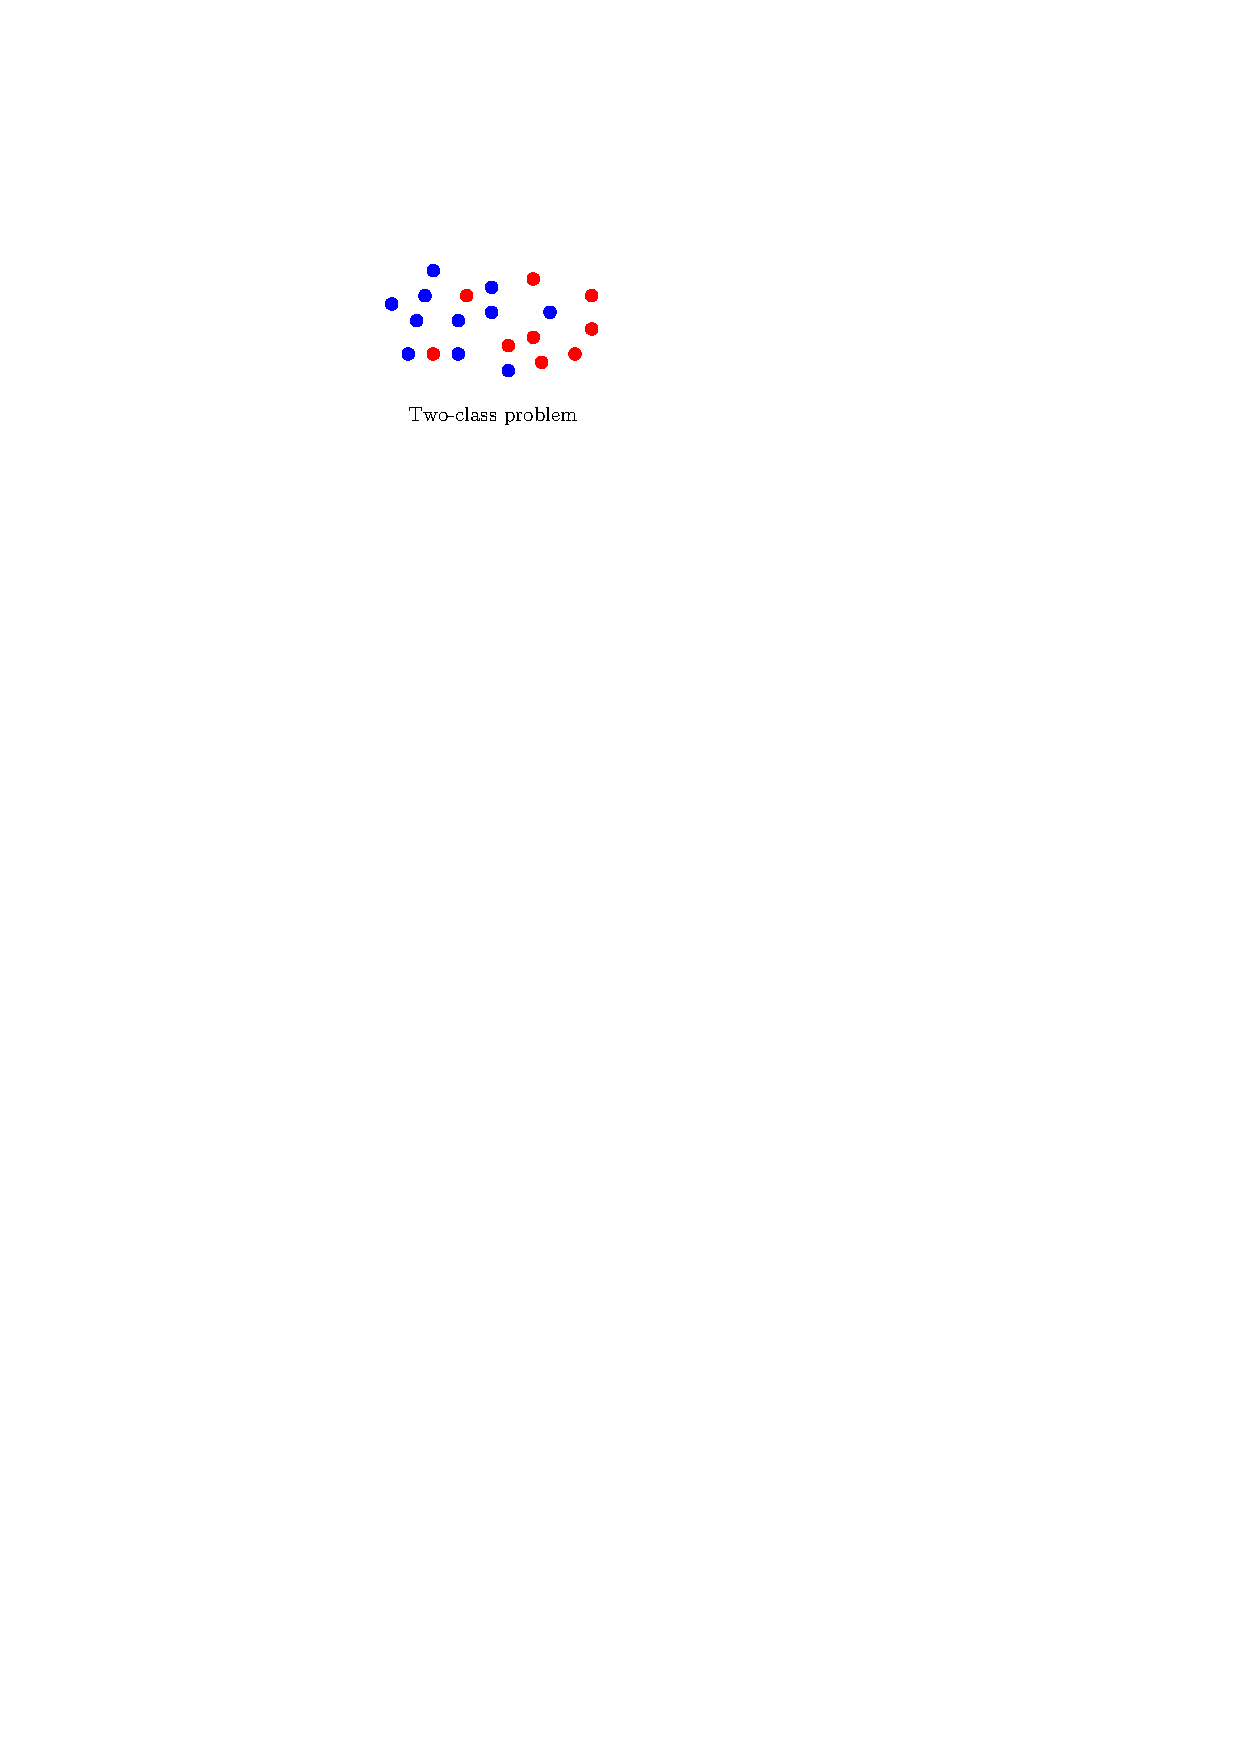
\includegraphics[width=0.32 \textwidth]{Fig1} \hspace{1.5cm} \pause
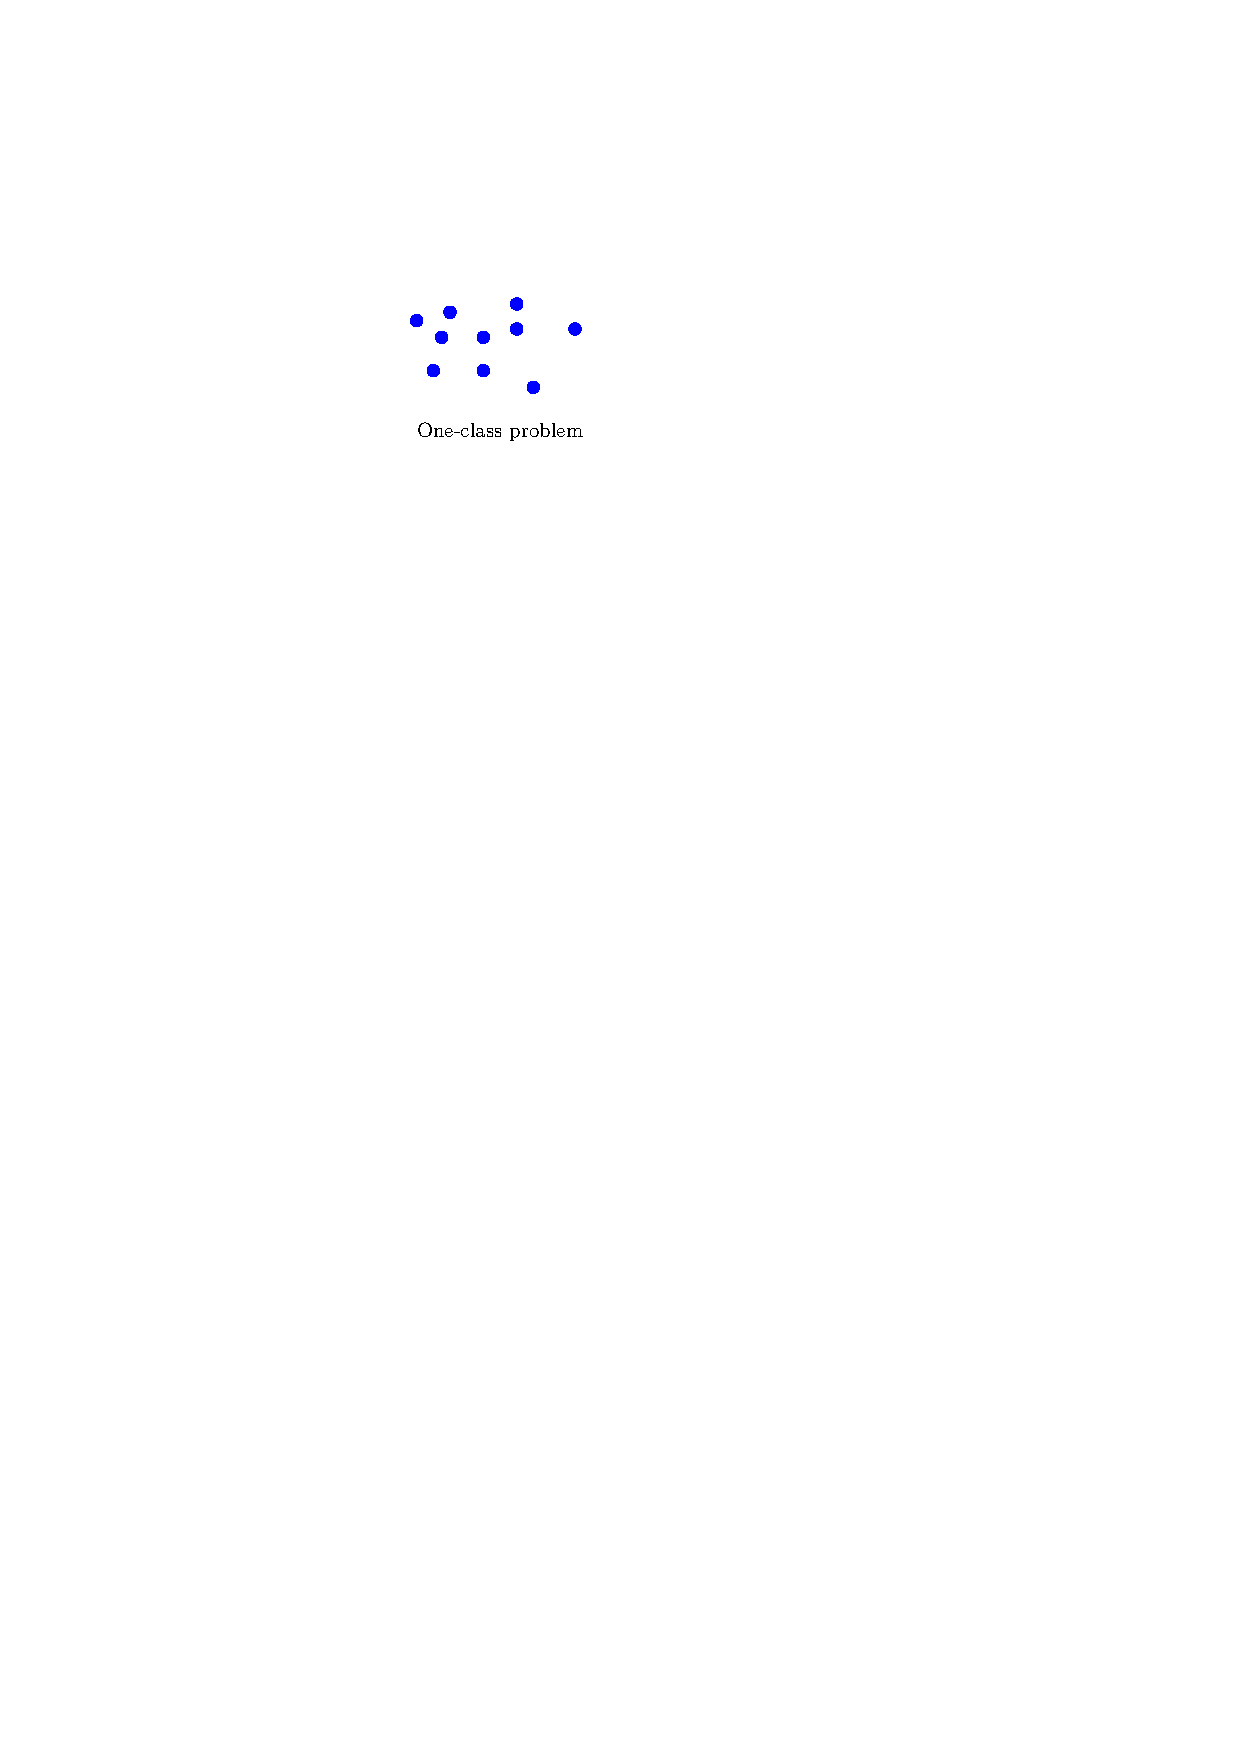
\includegraphics[width=0.27 \textwidth]{Fig2} 
\end{figure} \pause
\begin{block}{Learning from implicit feedback}
Learning from one-class problem, i.e. we are given only positive examples.
\end{block} 
\end{frame}


\begin{frame} 
\frametitle{Approaches} \vspace{-7mm}
\begin{block}{}
\begin{itemize}

\item Pointwise approach \\
{\footnotesize Solve a binary classification problem to predict if a user prefers an item \\
Model: trying to estimate $p(y=+1|u,i)$} 
\begin{itemize} \pause
\item {\color{blue} Advantage}: efficiency
\item {\color{red} Disadvantage}: ranking ineffectiveness 
\end{itemize} \pause \vspace{1mm} 

\item Pairwise ranking: \\
{\footnotesize A binary classification problem to predict which of any given two items a user will prefer}
\begin{itemize} \pause
\item {\color{blue} Advantage}: ranking effectiveness 
\item {\color{red} Disadvantage}: severely inefficient due to the quadratic computational cost (i.e. problematic in large-scale setting)
\end{itemize} \vspace{1mm} \pause

\item Special case: IRGAN 
\begin{itemize}
\item {\color{blue} Advantage}: provides an optimized negative sampler using SGD
\item {\color{red} Disadvantages}: \\
(1) difficult to tune hyper-parameters (2) inefficient training
\end{itemize} 
\end{itemize}
\end{block} 
\end{frame}

\section{This Work}

\begin{frame}
\frametitle{This paper} 
\begin{block}{Bayes rule}
$$p(y=+1|u,i) = \frac{p(i|u, y=+1) p(y=+1|u)}{p(i|u)}$$ \pause
\end{block}
\begin{block}{Estimating pdf of positive items for each user using MLE}
\begin{itemize}
\item {\color{blue} Advantages}: is efficient and effective in ranking
\end{itemize} 
\end{block} 
\end{frame}

\subsection{Problem Formulation}
\begin{frame}
\frametitle{Notation} 
\begin{block}{}
\begin{itemize}
\item[$\cal{U}$]: users; ${\cal{U}} = \{u_j\}_{j=1}^N$
\item[$\cal I$]: items; ${\cal{I}} = \{i_j\}_{j=1}^N$
\item[data]: $N$ i.i.d user feedback logs $(u_1, i_1, y_1), \ldots, (u_N, i_N, y_N)$ 
\item[y]: binary labels, $y \in \{+1, -1\}$. But here $y_j=1$ for all $j$. \\ 
{\footnotesize In implicit feedback we can observe only positive samples.}
\item[task]: Given a user, a ranker sorts items in the order in which they are most likely to interact with the user. 
\item[model]: modelling $p(i|u, y=+1)$ or simply $p(i|u)$.
\end{itemize} \vspace{3mm}
\end{block} 
\end{frame}


\subsection{Personalized Ranking}

\begin{frame}
\frametitle{Modelling the problem (personalized ranking)} 
\begin{block}{Using exponential family of distributions}
$$p_f(i|u) := p_0(i) e^{f_u(i) - A(f_u)}$$
parameterized by $f_u$. \vspace{3mm}
\begin{itemize} \pause
\item $p_0$: prior density function on $\cal I$, \pause  \vspace{1mm}
\item $f_u(i)$: the scoring function to learn ($u$'s preference score for $i$), \pause  \vspace{1mm}
\item $A(f_u) = \log \int_{\cal I} p_0(i) e^{f_u(i)} di$ (normalization: $\int_{\cal I} p_f(i|u) di = 1$), \pause  \vspace{1mm}
\item Assumption: $p_0$ uniform distribution, \pause \vspace{1mm}
\item $p_f(i|u) \propto e^{f_u(i)} \Longrightarrow p_f(i|u) =^{rank} f_u(i)$
\end{itemize}
\end{block} 
\end{frame}


\subsection{Personalized MLE}


\begin{frame}
\begin{block}{Risk} \vspace{-4mm}
$$R(f) = \E_u\Big[\hspace{-5mm} \underbrace{\underbrace{\hat{\E}_+}_{\color{blue} \text{\tiny{empirical $\E$ over + items}}}}_{\color{magenta} \hat{\E}_{p(i|u, y=+1)}} \hspace{-8mm}[-\log p_f(i|u)] + \underbrace{\underbrace{KLD\big(p_f(\cdot |u) || p_0(\cdot)\big)}_{\color{blue} \text{\footnotesize{Personalization term}}}}_{\color{magenta} \text{\tiny {incorporates both + and - items}}}\Big]$$ \pause \vspace{-5mm}

$$R(f) = \E_u\Big[\hat{\E}_+[-f_u(i)] + \hspace{-10mm} \underbrace{\E_{p_f(i|u)} [f_u(i)]}_{\color{blue} \to \text{\tiny negative instances in pairwise and pointwise}}\hspace{-10mm}\Big]$$  \pause \vspace{-5mm}

$$R(f) = \E_u\Big[\hat{\E}_+[-f_u(i)] + \frac{\E_{p_0}[f_u(i) e^{f_u(i)}]}{\E_{p_0}[e^{f_u(i)}]}\Big]$$ \pause \vspace{-3mm}

\end{block} 
\begin{block}{Risk Approximation}  \vspace{-8mm}
$$\hat{R}(f, {\cal{U}}_B, {\cal{I}}_B) = 
\underbrace{\frac{1}{|{\cal{U}}_B|} \sum_{u \in {\cal{U}}_B}}_{\color{blue} \E_u} \bigg(\underbrace{- \frac{1}{|{\cal{I}}_u^+|} \sum_{i \in {\cal{I}}_u^+} f_u(i)}_{\color{blue} \hat{\E}_+[-f_u(i)]} + \frac{\sum_{i \in {\cal I}_B} f_u(i) e^{f_u(i)}}{\sum_{i \in {\cal I}_B} e^{f_u(i)}}\bigg)$$
\end{block} 
\end{frame}


\begin{frame} 
\frametitle{Relation to IRWGAN} 
\begin{block}{Min-Max objective of IRWGAN for user $u$:} \vspace{-3mm}
$$\min_{q_u \in {\cal P}} KLD(q_u || p_0) + WD(P_u || Q_u)$$  \pause \vspace{-2mm}
$$= \min_{q_u \in {\cal P}} \Big\{ KLD(q_u || p_0) + \sup_{f_u \in {\cal F}} \Big[ \hat{\E}_+[f_u(i)] - \E_{q_u(i)}[f_u(i)] \Big] \Big\}$$ \pause \vspace{-2mm} 
$$ \overbrace{=}^{{\color{magenta} duality}} \sup_{f_u \in {\cal F}} \Big\{ \hat{\E}_+[f_u(i)] + \min_{q_u \in {\cal P}} \Big[ KLD(q_u || p_0) - \E_{q_u(i)}[f_u(i)] \Big] \Big\}$$ \pause \vspace{-3mm}
\begin{itemize}
\item[$\cal P$]: probability measures supported in $\cal I$  \vspace{-1mm}
\item[${\cal F}$]: a convex subset of 1-Lipschitz functions
\end{itemize} \pause  \vspace{-2mm}

$$R_{WGAN}(f) = \E_u\Big[\hat{\E}_+[-f_u(i)] + \hspace{-2mm} \underbrace{\E_{p_f(i|u)} [f_u(i)]}_{\color{blue} optimal \, q_u^*(i) \, = \, p_f(i|u)}\hspace{-2mm}\Big]$$ \pause  \vspace{-3mm}
$$\color{magenta}{R^*_{WGAN}(f)  = R(f)}$$  
\end{block} 
\end{frame}


\section{Experiments}

\begin{frame}
\frametitle{Datasets statistics and effectiveness (nDCG)}
\begin{figure}[h] 
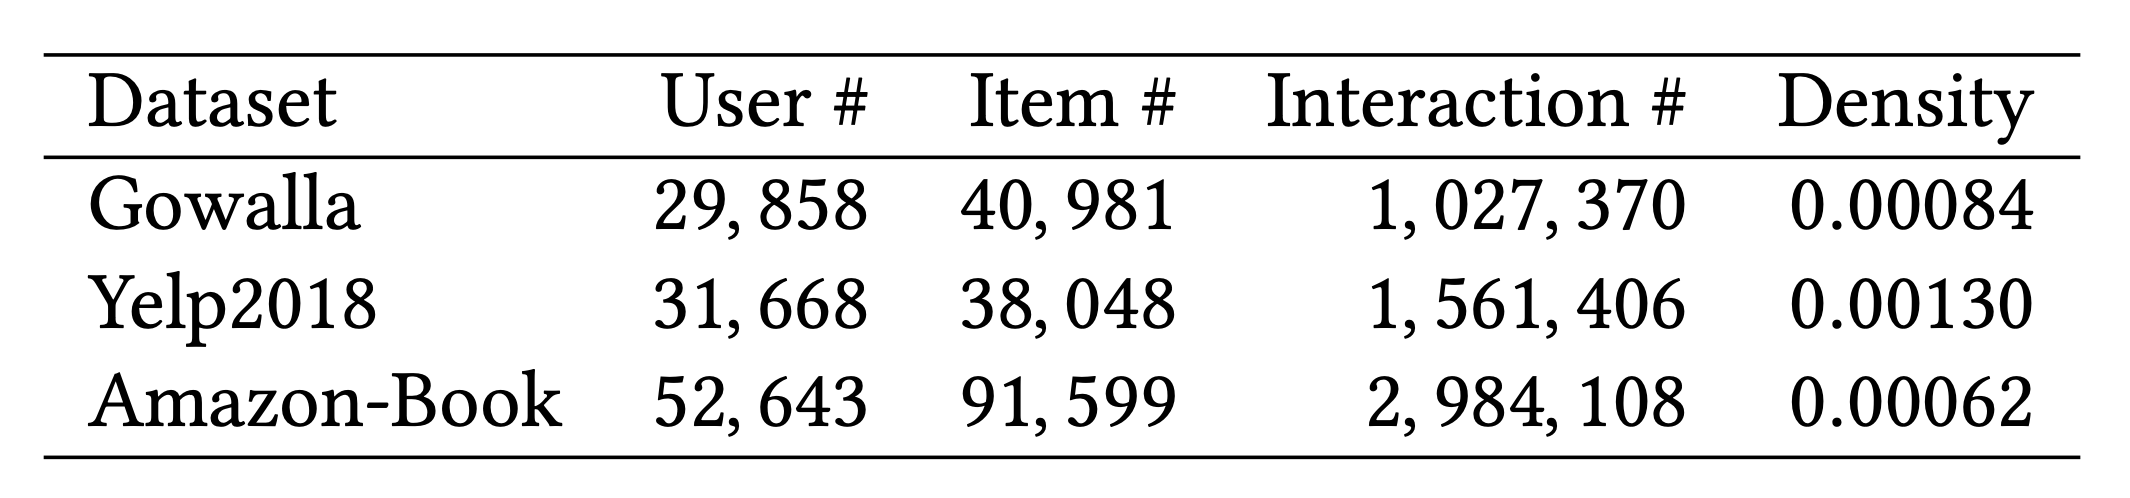
\includegraphics[width=0.85 \textwidth]{datasets} 
\end{figure} \pause

\begin{figure}[h] 
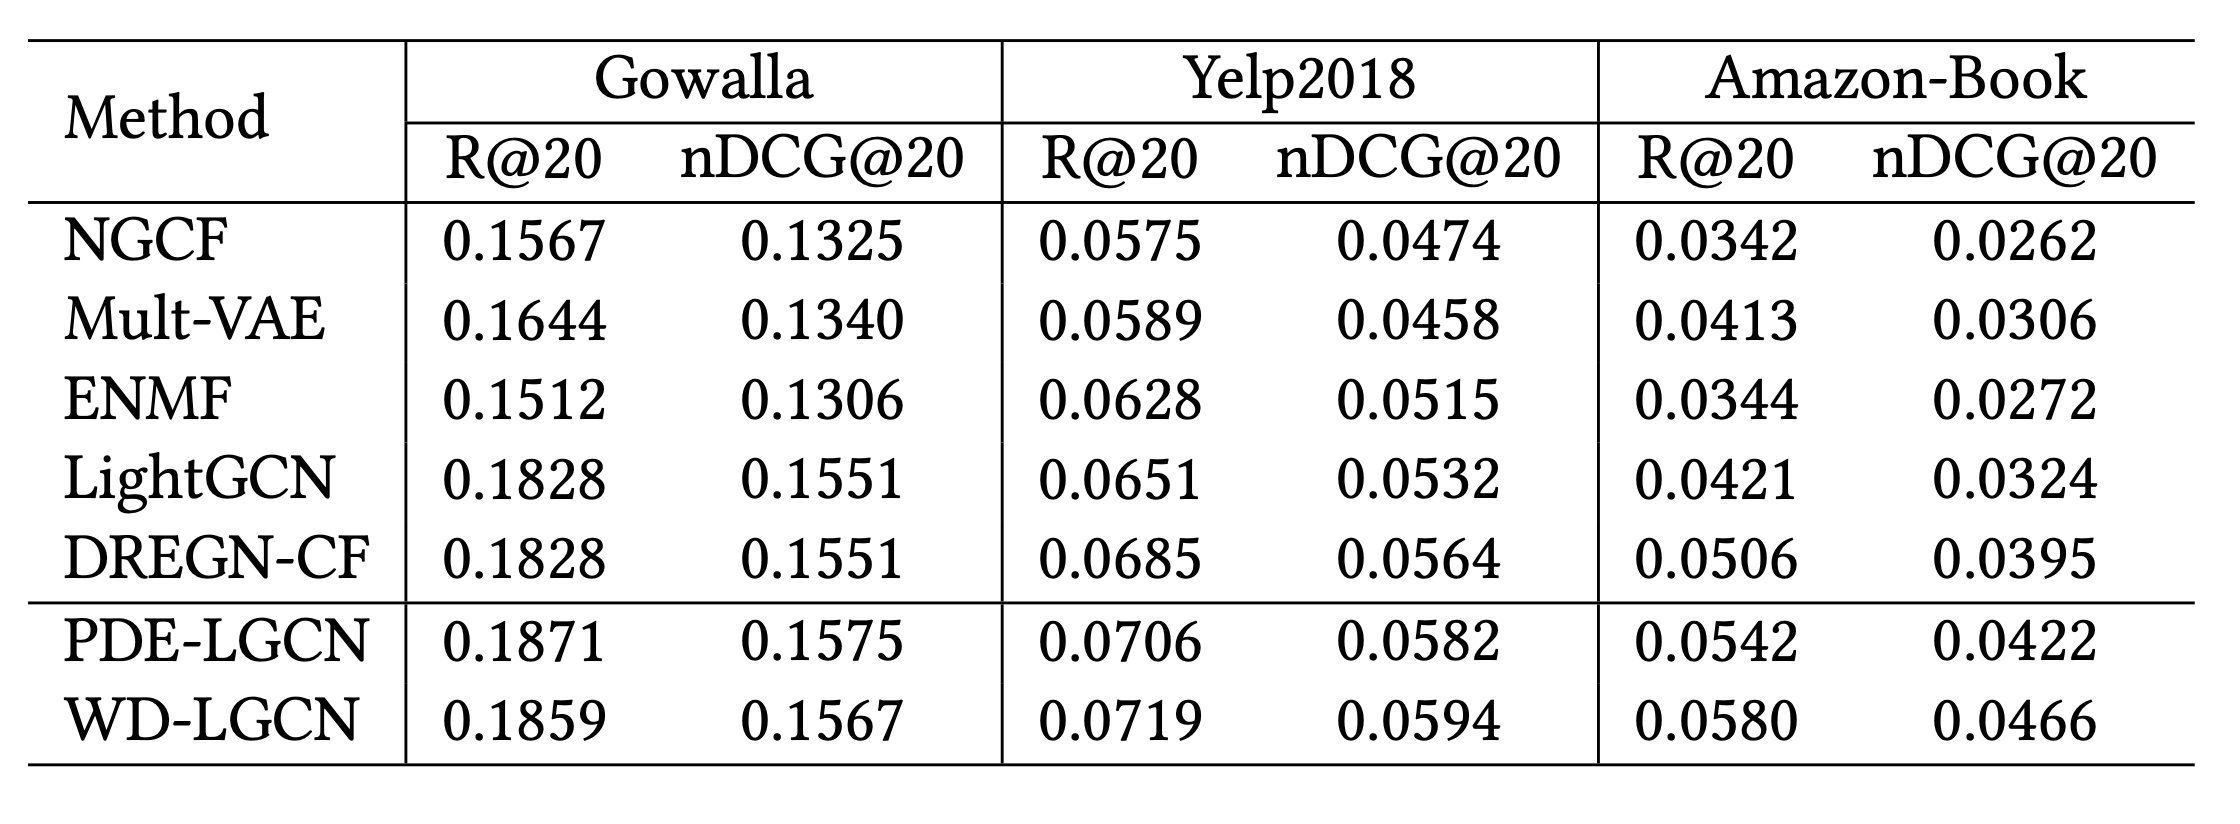
\includegraphics[width=1 \textwidth]{nDCG} 
\end{figure} \vspace{-2mm}
{\tiny{{\bf PDE-LGCN:} parametric density estimation LightGCN  \hspace{5mm}  {\bf WD-LGCN:} Wasserstein distance LightGCN}}
\end{frame}


\begin{frame}
\frametitle{Efficiency} \vspace{-2mm}
\begin{figure}[h] 
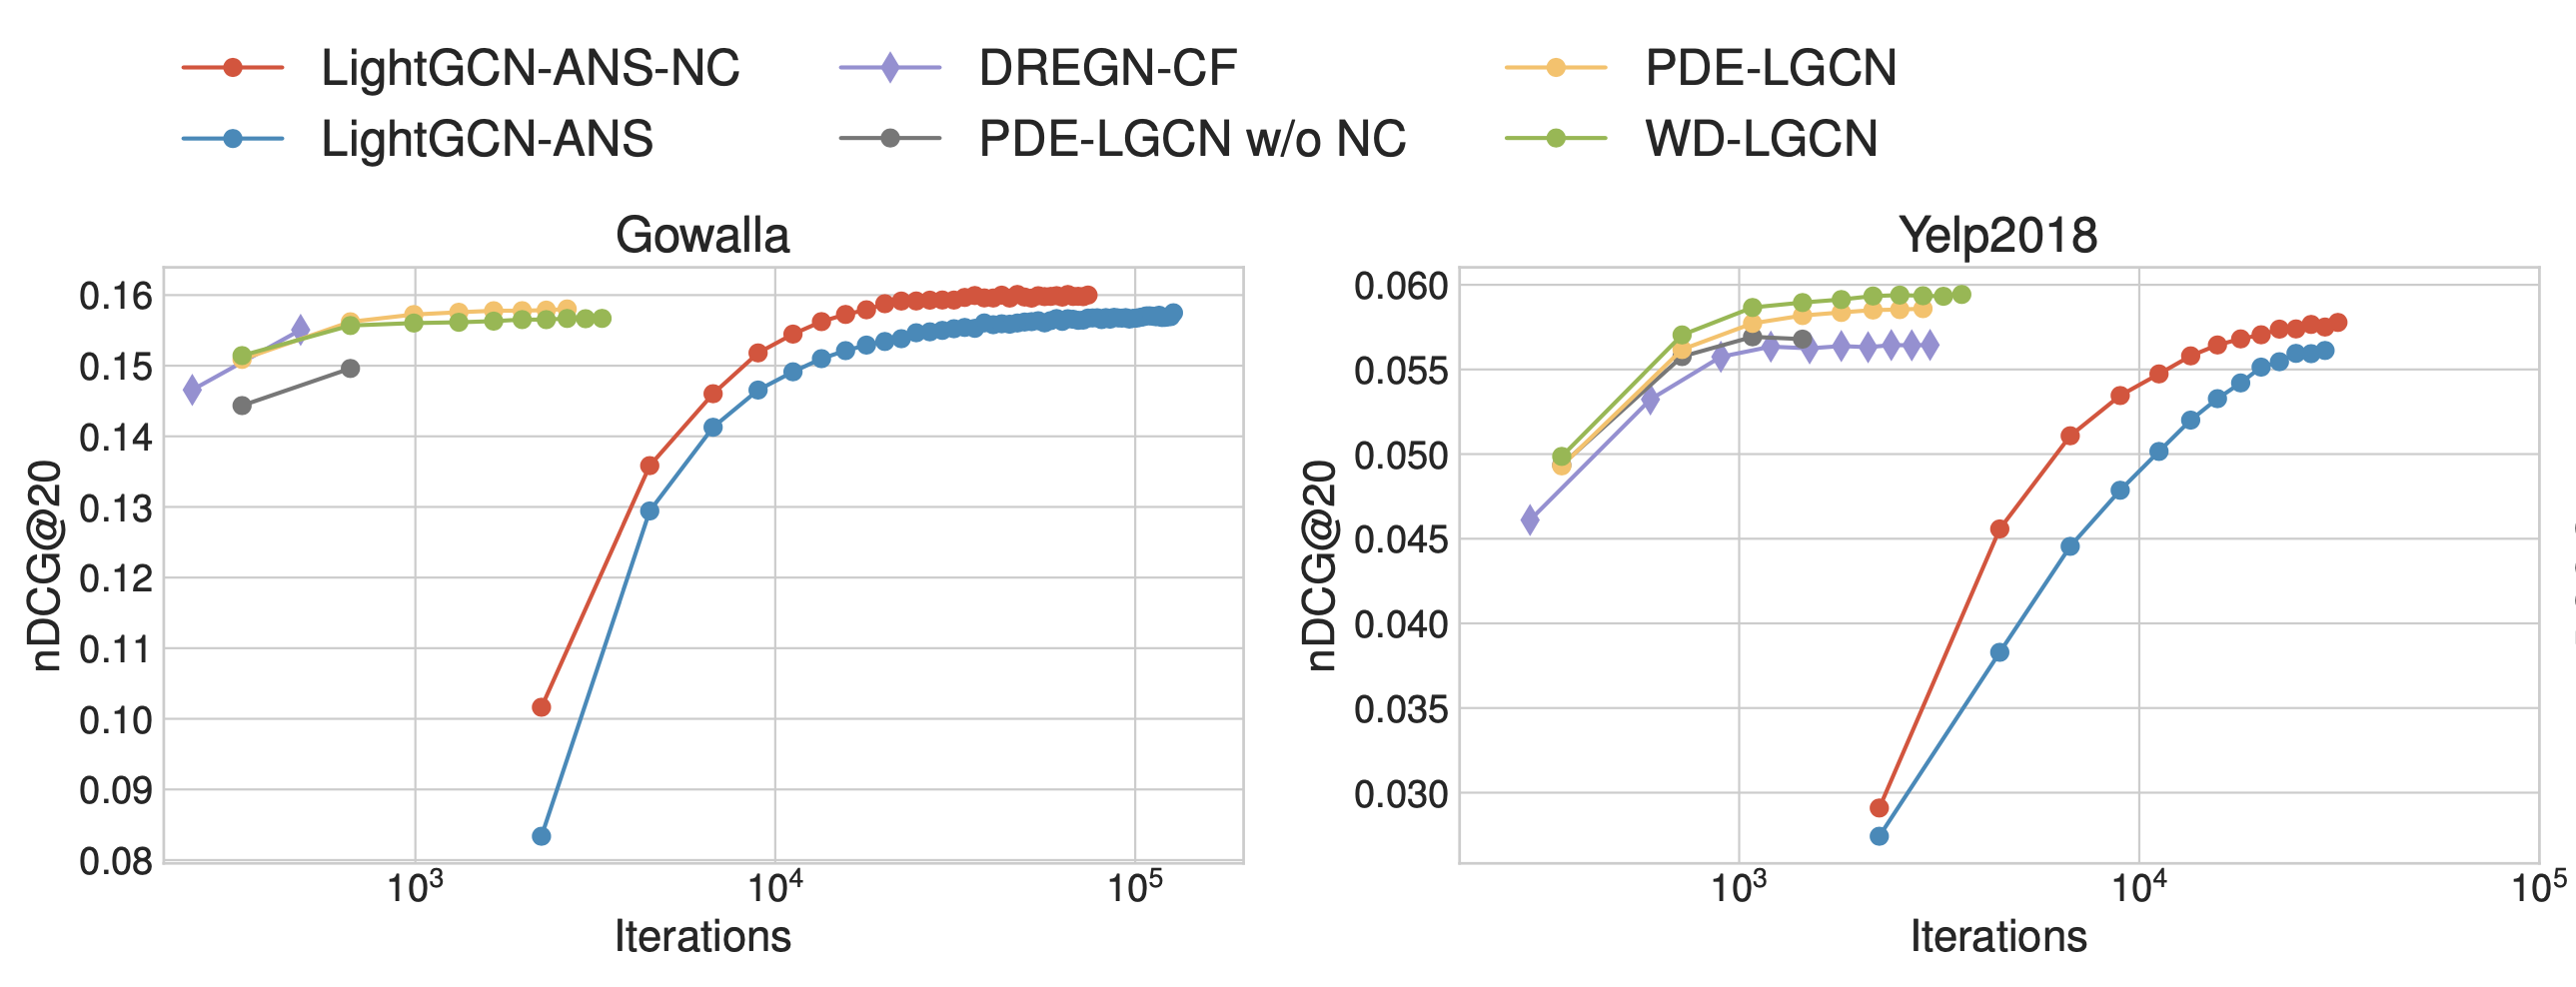
\includegraphics[width=1 \textwidth]{runtime1} 
\end{figure} \vspace{-5mm}

\begin{figure}[h] 
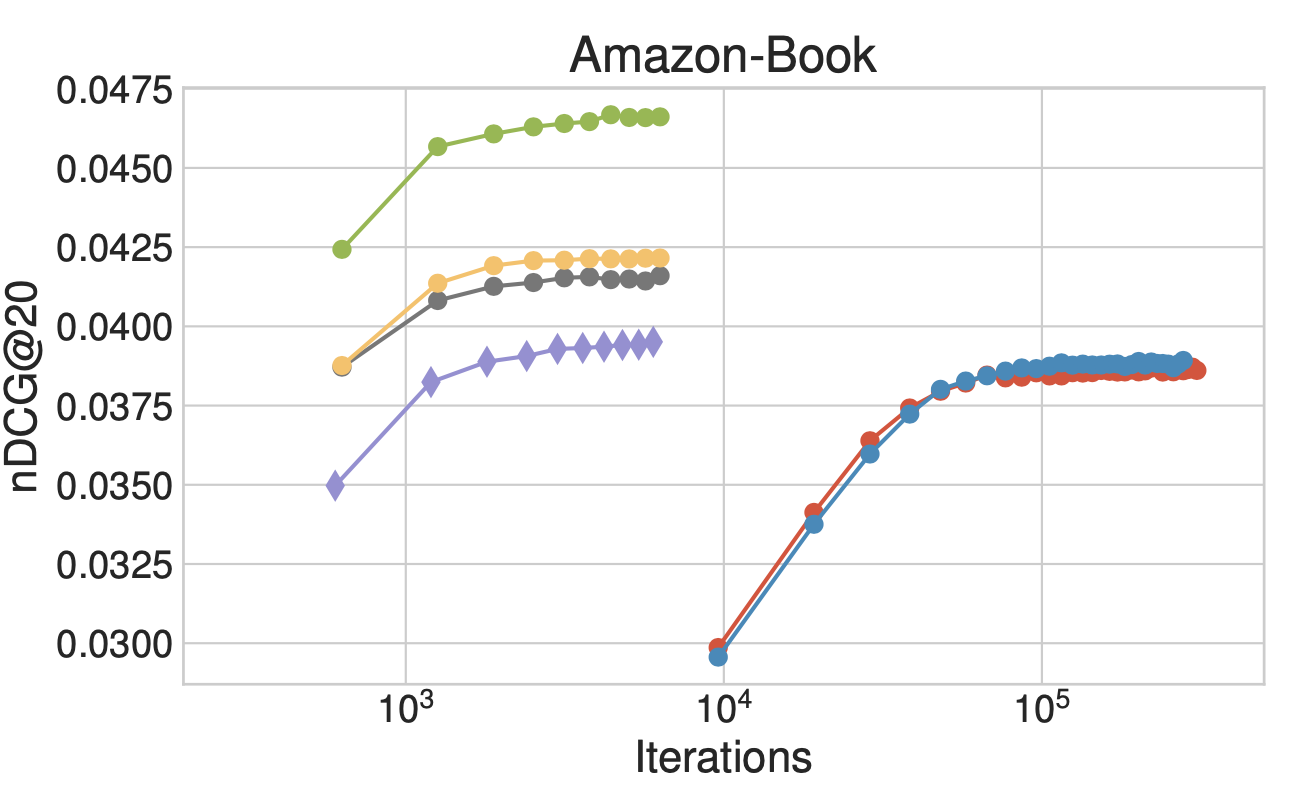
\includegraphics[width=0.5 \textwidth]{runtime2}
\end{figure} 
\end{frame}



\begin{frame}
\frametitle{nDCG in terms of clipping $n$} \vspace{-2mm}
\begin{figure}[h] 
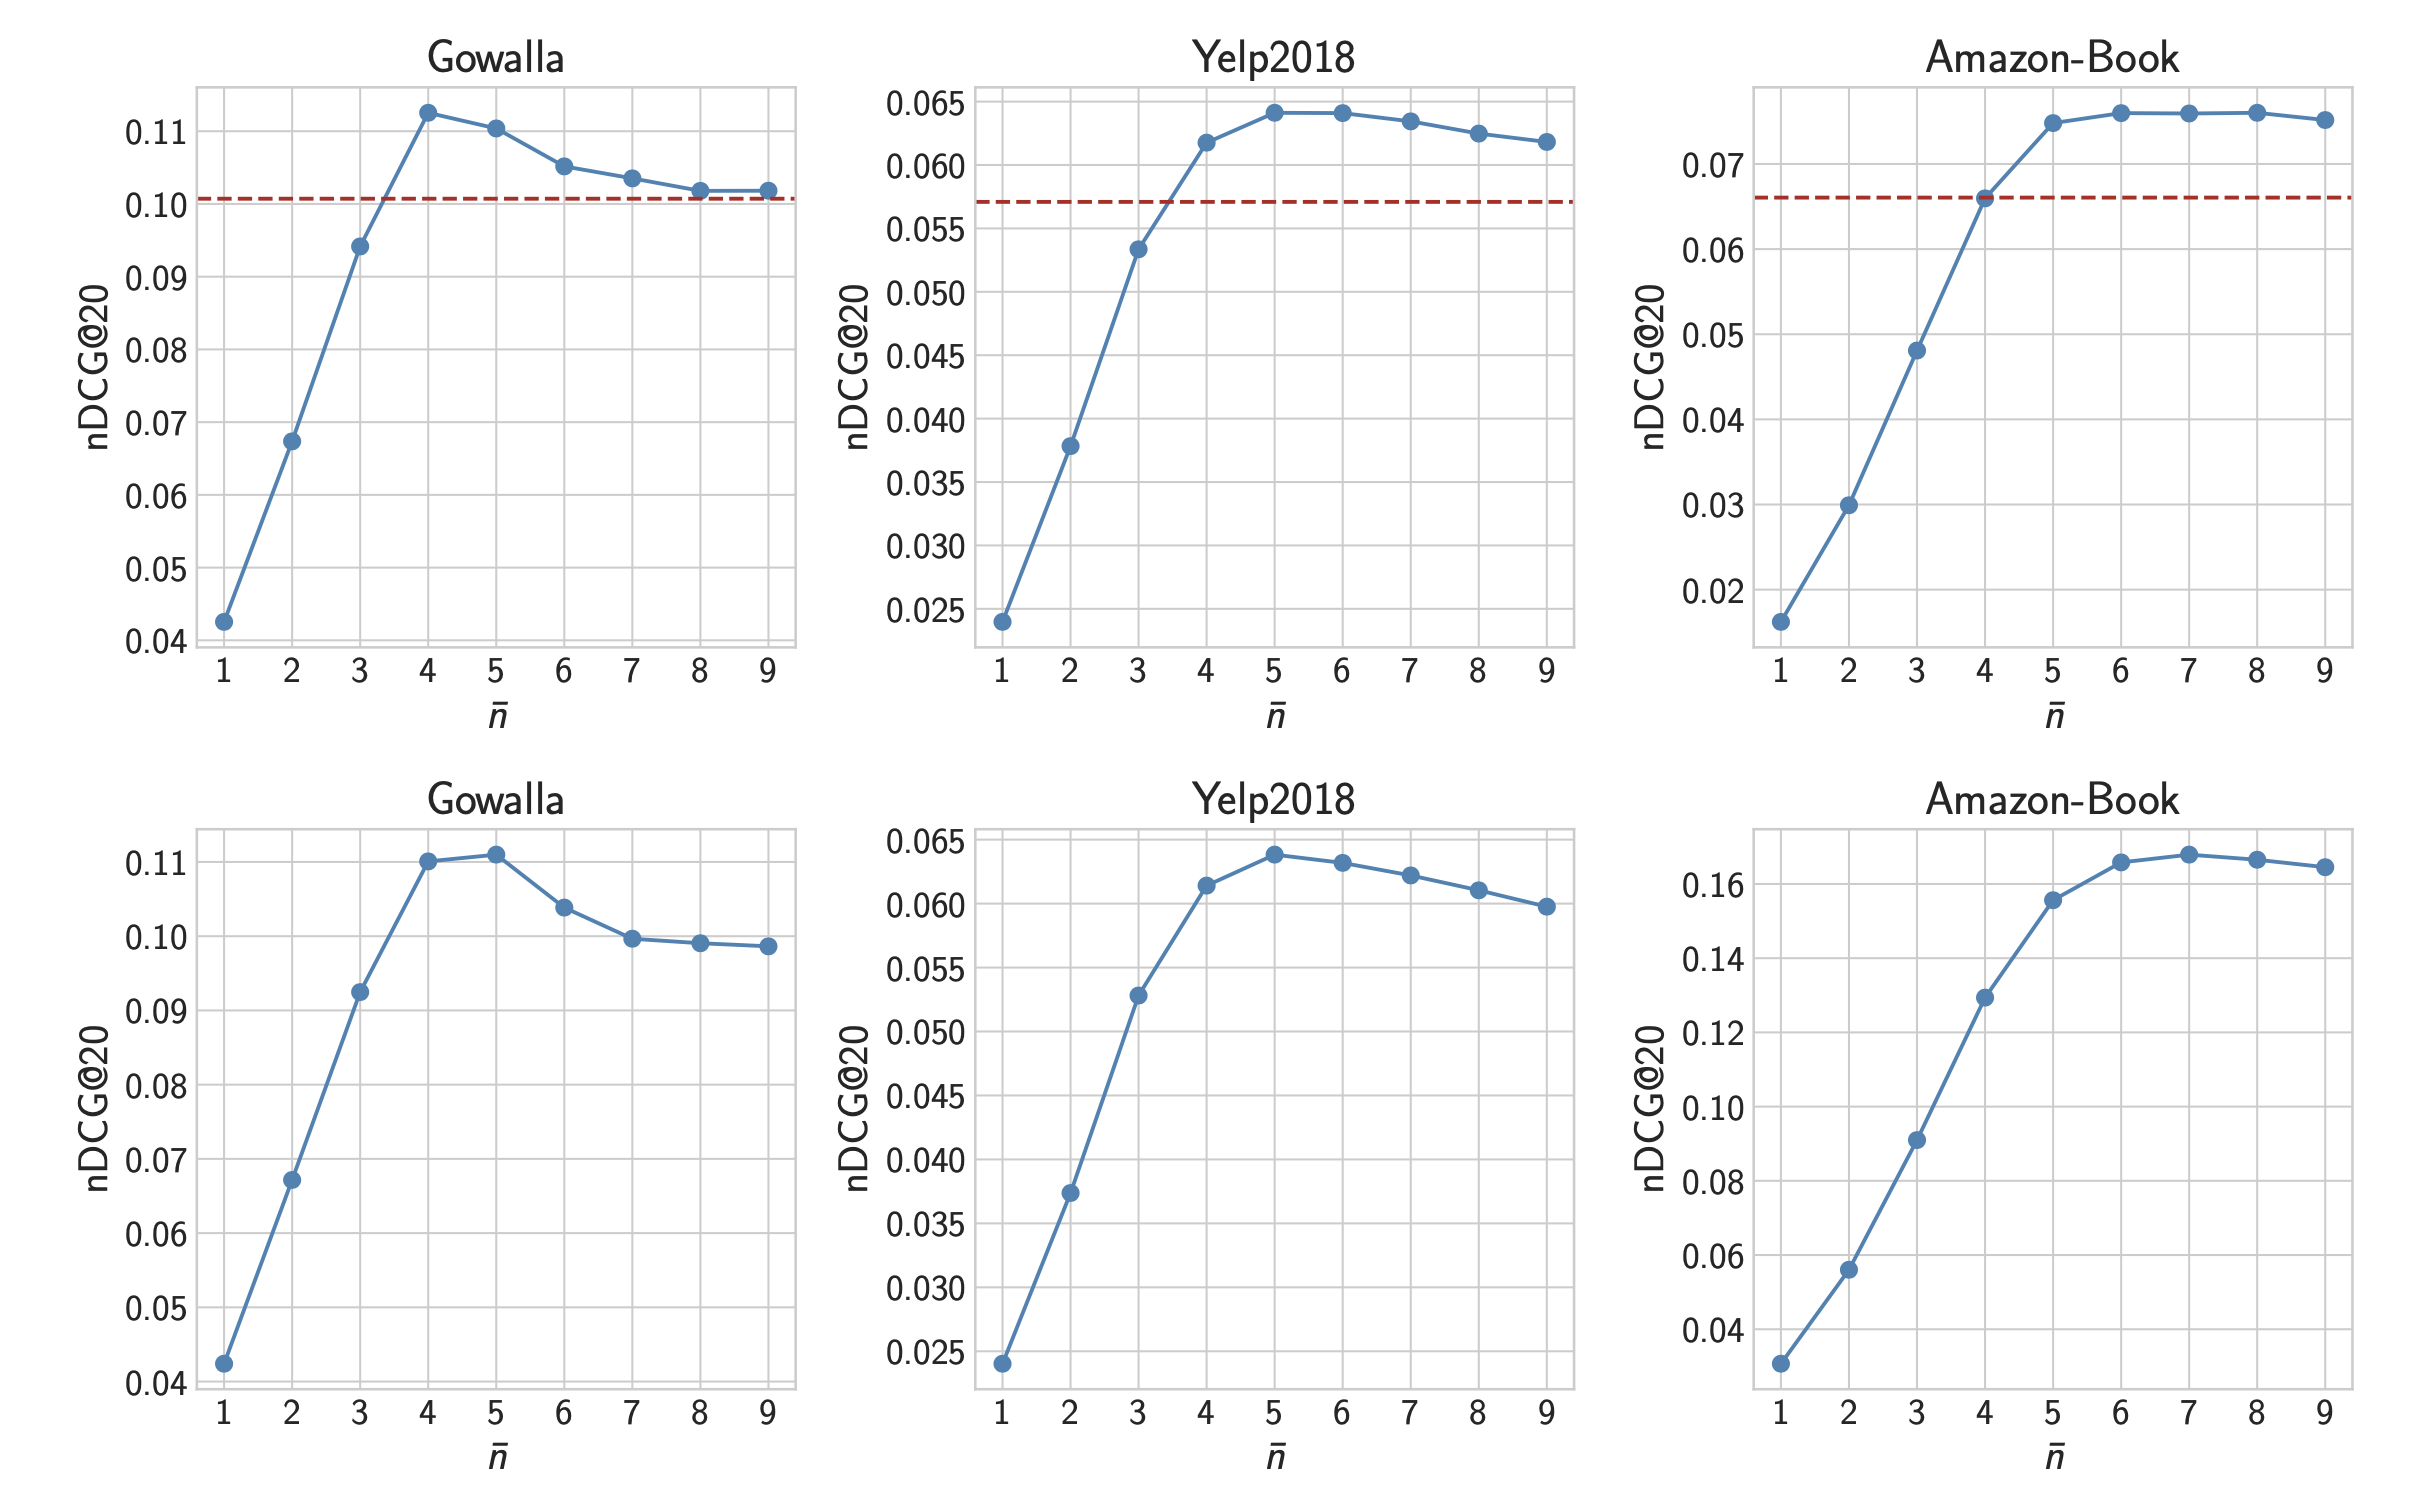
\includegraphics[width=0.9 \textwidth]{clipping-n}
\end{figure} \pause \vspace{-5mm}

\begin{figure}[h] 
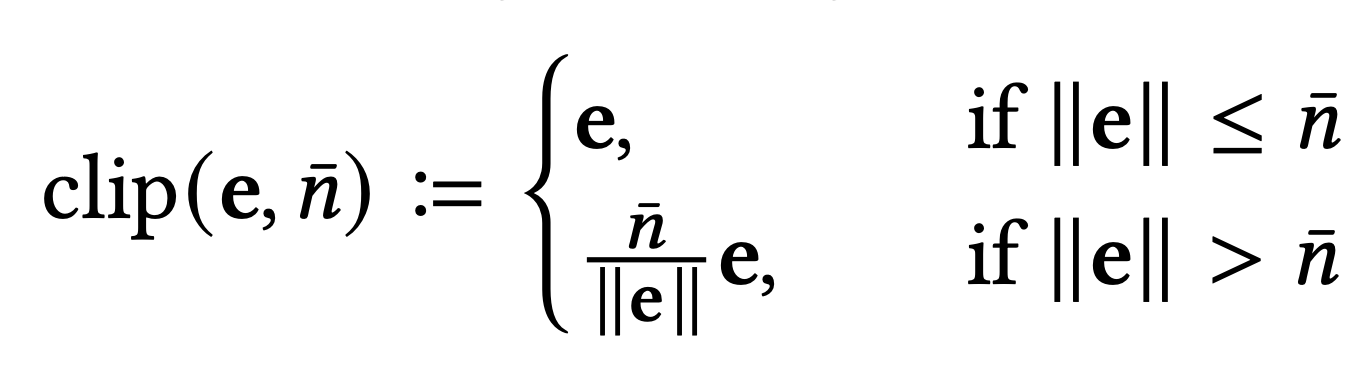
\includegraphics[width=0.4 \textwidth]{clip}
\end{figure}
\end{frame}


\begin{frame}
\frametitle{What I learned?}
\begin{itemize} \pause
\item We can learn from only positive labels (i.e. implicit feedback)! \pause
\item Density functions can help to learn efficiently and effectively. \pause
\item Exponential family of distributions is a powerful tool for learning to rank. \pause
\item Personalized term in loss functions can be done through KLD with uniform distribution which simultaneously encodes {\color{blue} +} and {\color{red} $-$} examples implicitly. 
\end{itemize}
\end{frame}


\section*{Questions}
{\color{white}1}
\begin{center} 
{\huge \color{magenta}{\sc \vspace{3cm} Questions?}}
\end{center}


\end{document}